% !Mode:: "TeX:UTF-8"
% !TEX program  = xelatex
\newgeometry{margin=1in}

\title{Assignment 6}


\section{Question 1}
\begin{statebox}{Timescale Invariance}{question-1}
    \begin{align*}
        S(t_{i+1}) &= S(t_i) + \mu\delta tS(t_i) + \sigma\delta tY_iS(t_i) \\S(t_{i+1}) &= S(t_i) + \mu\delta t^{1/4}S(t_i) + \sigma\delta tY_iS(t_i)
    \end{align*}
    Please verify or dispute the timescale invariance of the two models above by numerical experiments.
\end{statebox}

Therefore, we have the following code, which verifies the timescale invariance of the models by numerical experiments. And the result of the code below with the arguments $S_0=1$, $\mu=0.05$, $\sigma=0.5$, is Figure~\ref{F:1}.

\lstset{showspaces=false, showtabs=false, tabsize=2, framexleftmargin=5mm, frame=shadowbox, numbers=left, numberstyle=\tiny, breakautoindent=false}
\lstinputlisting[style=Matlab-Pyglike]{code/timescale_invariance_asset_path.m}

\begin{figure}[H]
	\centering
	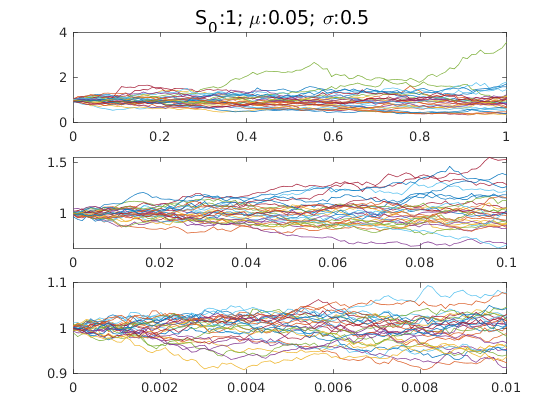
\includegraphics[width=\textwidth]{figures/2019-10-30-timescale-invariance.png}
	\caption{Timescale Invariance Asset Path}\label{F:1}
\end{figure}
